% This template was initially provided by Dulip Withanage.
% Modifications for the database systems research group
% were made by Conny Junghans,  Jannik Strtgen and Michael Gertz

\documentclass[
     12pt,         % font size
     a4paper,      % paper format
     BCOR=10mm,version=first,     % binding correction
     DIV=14,version=first,        % stripe size for margin calculation
%     liststotoc,   % table listing in toc
%     bibtotoc,     % bibliography in toc
%     idxtotoc,     % index in toc
%     parskip       % paragraph skip instad of paragraph indent
     ]{scrreprt}

%%%%%%%%%%%%%%%%%%%%%%%%%%%%%%%%%%%%%%%%%%%%%%%%%%%%%%%%%%%%

% PACKAGES:

% Use German :
\usepackage[english]{babel}
% Input and font encoding
\usepackage[utf8]{inputenc}
\usepackage[T1]{fontenc}
% Index-generation
\usepackage{makeidx}
% Einbinden von URLs:
\usepackage{url}
% Special \LaTex symbols (e.g. \BibTeX):
%\usepackage{doc}
% Include Graphic-files:
\usepackage{graphicx}
% Include doc++ generated tex-files:
%\usepackage{docxx}
% Include PDF links
%\usepackage[pdftex, bookmarks=true]{hyperref}
\usepackage{csquotes}

% Fuer anderthalbzeiligen Textsatz
\usepackage{setspace}

% hyperrefs in the documents
\usepackage[bookmarks=true,colorlinks,pdfpagelabels,pdfstartview = FitH,bookmarksopen = true,bookmarksnumbered = true,linkcolor = black,plainpages = false,hypertexnames = false,citecolor = black,urlcolor=black]{hyperref} 
%\usepackage{hyperref}


%%%%%%%%%%%%%%%%%%%%%%%%%%%%%%%%%%%%%%%%%%%%%%%%%%%%%%%%%%%%

% OTHER SETTINGS:

% Pagestyle:
\pagestyle{headings}

% Choose language
\newcommand{\setlang}[1]{\selectlanguage{#1}\nonfrenchspacing}

\usepackage{biblatex}
\addbibresource{references.bib}

\begin{document}

% TITLE:
\pagenumbering{roman}
\begin{titlepage}
     \vspace*{1cm}
     \begin{center}
          \vspace*{3cm}
          \textbf
          {
               \Large University of Heidelberg\\
               \smallskip
               \Large Institute for Computer Science\\
               \smallskip
               \Large Working group database systems\\
               \smallskip
          }

          \vspace{3cm}

          \textbf{\large Bachelor thesis}

          \vspace{0.5\baselineskip}
          {
               \huge
               \textbf{Messaging Architecture for Integration of Identity Management Systems}
          }

     \end{center}

     \vfill
     {
          \large
          \begin{tabular}[l]{ll}
               Name:                 & Jonas Gann              \\
               Matriculation number: & 3367576                 \\
               Supervisor:           & Prof. Dr. Michael Gertz \\
               Date of submission:   & \today
          \end{tabular}
     }

\end{titlepage}

\onehalfspacing

\thispagestyle{empty}

\vspace*{100pt}
\noindent
I assure that I have written this bachelor thesis on my own and only used the specified sources and resources and that I followed the principles and recommendations "Responsibility in Science" of the University of Heidelberg.

\vspace*{50pt}
\noindent

\underline{\phantom{mmmmmmmmmmmmmmmmmmmm}}

\medskip
\noindent
Date of Submission: \today
\newpage

\chapter*{Zusammenfassung}

\newpage

\chapter*{Abstract}

\newpage

\tableofcontents
\cleardoublepage
\pagenumbering{arabic}

\chapter{Context}
Since invention of the World Wide Web, the number of its users increased rapidly. Today, more than 90 percent of the German population use the internet \cite{Onlinestudie}. Enterprises and organizations, recognised this potential to provide their services to a large number of people as Service Providers (SP). A frequently used method of SPs is "online self-service" (OSS). Specialized software tools enable customers to use services through the internet without direct human interaction.

Many tools require identification of a user in case interactions or initiated business processes have to be associated with him. A system for management of identities of users therefore is part of numerous system architectures. Service Providers usually enable users to manage their partial identities using online self-service through so called User Profiles. Today, customers of SPs are associated with multiple partial identities and user profiles - one for each SP

The result is a digital identity crisis \cite{IdentityCrisis}:
\begin{itemize}
    \item Multiple SPs collect, use and share parts of identities which leads to a distributed and fragmented identity.
    \item As a result of the distributed identity, risk of data breaches increases.
    \item Managing multiple use profiles is very inconvenient for users.
    \item It is often unclear who stores which data and for what purpose.
    \item SPs have an incentive to collect and share more user data than they need, to provide their service.
\end{itemize}

An improved model for identity management is necessary. In recent years, multiple new models have been invented. One model called Social Login became popular. It enables customers to create User Profiles for SPs through existing User Profile of Social Networks like Facebook. This improves identity management by enabling SPs to rely on the external profile for unique identification, authorisation and personal attributes. Users can therefore manage identity related information through their Social Profile which is accessed by the SP.

This approach, however, still leaves the requirement of User Profiles for each SP because, depending on the provided service, additional attributes which are not part of the Social Profile, have to be manageable by the user. SPs also might require additional online self-service tools the social network does not provide.

The solution to this problem is an Identity Management Provider (IMP) which manages the whole online identity of a person and can replace the individual partial identities and User Profiles. The system itself is provided and hosted by a SP for consumption by other SPs. To replace existing User Profiles, the IMP can not only rely on systems for registration, authentication, authorisation and provisioning. Additional requirements of SPs like communication, data wallet and management of additional attributes have to be satisfied.

In order for an SP to use identities and services of an IMP, an integration into the system architecture of the SP has to take place. Due to the complex nature of system architectures and identity management, this is a difficult task.

A currently relevant example for usage of online self-service with particular interesting requirements for identities is the German "Online Access Law" (Online Zugangs Gesetz: OZG). It requires all administrative services of the German federal republic, each member state and commune to be digitally available through interoperable user profiles. The current plan is to make the profiles only available for usage in context of the OZG. From a user perspective, this would be yet another partial identity and user profile to manage.

\chapter{Objective}
Based on the prominent example of the OZG, the bachelor thesis will construct a message based integration architecture which enables system architectures of service providers with existing user profiles to make their services usable with an Identity Management Provider. In order to make the integration architecture suitable to real life requirements, the OZG is selected as an example due to its current relevance and high requirements regarding identity management. The integration architecture is however not only applicable in cases relevant for OZG but also for other Service Providers with similar requirements. As requirements of SPs are not guaranteed to be similar to those of the OZG, the integration architecture is built to be expendable.

The \textbf{integration architecture} for the OZG enables \textbf{IMP functionalities} to be usable for selected \textbf{OZG scenarios} by integrating a \textbf{connector} in the \textbf{system architecture} of a member state.

\begin{itemize}
    \item OZG scenarios are based on documented digitalization efforts of administrative services in the context of the OZG and are for example be the application for an administrative service or the communication with a governmental institution.
    \item The system architecture is based on documentation about architecture plans of member states.
    \item The functionalities of the IMP are based on a requirements analysis of OZG scenarios and additional research.
    \item The connector is defined based on functionalities the integration architecture requires from the IMP.
    \item The integration architecture is the main scientific contribution of this bachelor thesis. It is based on messaging patterns in order to utilize a combination of established and tested messaging solutions. In order to save investments it also reuses as many system components as possible and modifies as few system components as necessary.
\end{itemize}

\chapter{Structure of Work}
In the beginning of the thesis, terminology and basic concepts are explained.
This includes definitions of terms like Online Self-Service, Identity and Identity Management. The concept of Identity Management Providers and the Online Access Law are explained. The special relevance for integration of IMPs and OZG are described.

Then, preparatory work relevant for the integration architecture is presented. Relevant OZG scenarios based on digitisation documentations of administrative services are analyzed in order to define important features the IMP is required to have. The connector which makes the IMP accessible towards the integration architecture is documented. Based on documentation of system architectures of several member states, relevant components of the architecture relevant for the OZG are selected. Each component is explained in detail along with the functionalities it provides for usage by the integration architecture.

The integration architecture integrates previously documented connector and components of the system architecture in order to make selected OZG scenarios usable with the IMP. The architecture is presented iterative. Each iteration contains increasingly demanding requirements along with the documentation of the increasingly complex integration architecture. Each documentation is done through textual explanations, multiple flow diagrams and one messaging architecture.

In order to validate the integration architecture, the execution of one administration service with usage of the IMP is evaluated in theory.

\chapter{Fundamentals}

\section{Terminology}

\subsection{Service Provider}
Service providers (SP) are entities like enterprises or organisations which make services accessible over the internet.

\subsection{Online Self-Service}
Online self-service (OSS) describes a method used by Service Providers to make their services available to the user. The method is characterized by being available over the internet, requiring no direct human interaction but instead enabling the user to access services in a self-reliant way. The user is usually supported by a variety of software solutions.

\subsection{Self-Service Tools}
Self-service tools are software solutions for customers to enable a online self-service experience. Depending on the use case, the tools can be transactional or informing. Informing tools help users to retrieve relevant information, often replacing human customer support. Transactional tools help users to interact with services in a persistent way to for example save personal data or trigger business processes.

Information tools can be for example so called "WiKi" pages or search fields which assist the user in his process of finding information. Transactional tools can be for example online forms which assist the user in his process of triggering an order placement business process.

In contrast to information tools, transactional tools often require identification of users in order to associate them with changes they made to the system: If a user triggers the business process of ordering a product, the SP requires identification of the user.

\subsection{Digital Identity}
The digital identity, for simplicity called identity in the thesis, is the sum of all digital personal information. This includes a set of identifiers which are pieces of information that can uniquely identify an entity and attributes which describe properties of an entity but do not uniquely identify it. It is also possible to use an aggregation of attributes as identifier.

Identifiers which are commonly used by SPs are the phone number and E-Mail address. Attributes are for example nicknames, hobbies, interests or education. The full name of a person is often not sufficient unique identification, the aggregation of name, age and home address can therefore be used as identifier.

\subsection{Partial Digital Identity}
A partial digital identity is a subset of an identity. Partial identities are commonly used by SPs to manage identity information which is relevant for them. 

\subsection{Identity Management}
Identity management is the creation, utilization / reading , updating and deletion of identities or partial identities. The possible utilization of identities depends on the system for management of identities. It could be for example authorization for a service or communication through an inbox.

\subsection{Identity Management System}
Identity management systems are solutions which enable SPs and customers to manage identities.

\subsection{User Profile}
User profiles are one method for identity management. They are characterized by each SP providing a separate identity management system which often consist of an identity provider (IdP) for storing identities, a customer relation management system (CRM) for accessing identities internally and a website with online self-service tools for providing access to customers.

\section{Digital Identity Crisis}
The current situation of digital identities has the following core issues:
\begin{itemize}
    \item aktuelle übersicht über identitiy management
    \begin{itemize}
        \begin{itemize}
            \item oAuth
            \item saml
        \end{itemize}
        \item Social Login
        \item central idps
        \item idendity federation (SOcial login, Single sign on)
        \item device identity kopplung
        \item SSI
    \end{itemize}
\end{itemize}

\section{Identity Management Provider}
Identity management providers (IMP) are a method for identity management which aims to solve the digital identity crisis. They are characterized by giving SPs access to customer identities for which they provide one-stop online self-service. The important aspect of IMP is, that the identity is stored and managed in one place and its utilization is enabled through integration with system architectures of multiple SPs.

\subsection{Objective}
The IMP method can solve the identity issues the following way:

\subsection{IMP System}
A system for IMP can work as follows:

Additional requirements for IMP systems can exist and are analyzed as part of the preparatory work.

\subsection{Integration}
The IMP system has to be integrated. A connector is used:

\subsection{Challenges}
The IMP system has the following problems / open questions regarding integration:
\begin{itemize}
    \item which personal information resides at SP systems an which at IMP systems? => data the user personally manages resides at IMP systems, derived data etc. at SP systems
    \item should data be mirrored at the SP and just a synchronisation functionality exist
\end{itemize}

\section{Online Access Law}
The Federal Ministry of the Interior, Building and Community is, amongst other things, responsible for modernizing public administration \cite{BMI:Moderne_Verwaltung}. Current modernization efforts lie in the construction of an E-Government \cite{BMI:Behoerdengaenge}.
The E-Government-Law in 2013 was an early step increasing internal usage of digital systems in governmental administration. This includes for example the usage of digital personal files and scanning of documents for replacement \cite{BMI:E-Government_Gesetz}. 
In 2017 the German government passed the law for improvement of online access to administrative services (OZG) which focuses on usage of administration services by the people \cite{BMI:Onlinezugangsgesetz}. 
Modernization of the administration, however, is not exclusive to Germany as in 2018 the European Parliament and Council decided on a Single Digital Gateway (SDG) providing uniform access to digital administrative governmental services of every European country \cite{BMI:Single_Digital_Gateway}.

Customers on the free market are used to One-Stop-Shops providing access to services of companies in one digital place. Many self-service methods improve the user experience: Customers of e-commerce companies can put products in a digital shopping card, pay with digital money and select a location for delivery. In most cases, no direct human to human interaction is required. Customers complete the process of ordering in self-service. The progress of online self-service usage on the free market is a result of the ongoing digitalization of the world and the competitiveness of the market. Today, many customers own personal computers or smartphones and companies providing easy access to their services via online self-service have an advantage in the market.
Governmental institutions provide administrative services for customers. This can for example be an application for child benefit or a new ID card. In contrast to the free market, access to administrative services is, in most cases, not available through online self-service. Reasons are, that digitalization is expensive and governmental institutions do not have competitors.
Digitalization of governmental administration could for example enable users to inform themselves about available administrative services and access them over the internet. The need to personally appear in offices of an administration would be reduced. Communication about questions or required documents could also happen faster, more immediate, and more reliable over the internet than over mail. Governmental institutions could reduce bureaucracy through modernization of registries and the once-only principle.
The German government recognizes the possible improvements and presents, amongst other things, the OZG as a solution. \cite{IT-Planungsrat:Herausforderung}

The law for improvement of online access of administrative services (Online Access Law - OZG) passed in 2017 and requires federal republic and member states to execute the following regulations until 2022 \cite{BMI:OZG_Wortlaut}:
\begin{enumerate}
    \item \textbf{Digital availability of administrative services} \\
    An administrative service is the electronic processing of administrative procedures which are available from outside the governmental institution.  As it is not clear which administrative services exactly are meant by the definition of the OZG, the BMI created a catalogue \cite{BMI:Verwaltungsleistungen}. The OZG requires these services to be digitally available. As a guideline to what is considered sufficient availability, the BMI defined a maturity model \cite{BMI:Digitale_Services}.
    \item \textbf{Digital access to administrative services through administration portals of a portal network} \\
    Federal republic, each member state and each commune must provide an administration portal. Portals of communes must be linked to the portal of the corresponding member state. Portals of federal republic and member states must be connected through a portal network. \cite{BMI:Portalverbund} Each portal must provide a "seek and find" feature, which enables users to find all administrative services provided by any administration portal \cite{Cotar:Drucksache_19/19089}. 
    \item \textbf{Interoperable user profiles for accessing administrative services} \\
    Federal republic and member states must provide user profiles which can be used to identify the corresponding person while requesting access to administrative services, to save personal information according to the once-only principle, to receive and send messages via a digital mailbox and to pay for services \cite{Cotar:Drucksache_19/19089}. The user profiles must be interoperable for every administration portal of the portal network.
\end{enumerate}

Execution of the OZG can be separated into two projects: Digitalization and Networking. Digitalization focuses on transformation of existing processes and services to be using modern technologies. This includes most importantly the digitalization of governmental administrative services. The networking focuses on connecting existing and future governmental systems to make digitalization universally usable. This includes most importantly the construction of administration portals which are connected in a portal network.

Many services, which are still bound to paper must be digitized. In total, the BMI lists 575 relevant services. Some of them are provided by the federal republic, some by the member states and yet other by the communes. Respective to these responsibilities, the task of digitalization is distributed between federal republic and member states, where each member state is assigned to take the lead for specific areas. \cite{BMI:Onlinezugangsgesetz} Results of the digitalization are documented on the "OZG-Informationsplattform" \cite{BMI:Informatiosplattform} as process diagrams and data schemata.

Administrative services are made available through administrative portals which are be provided by federal republic, each member state and each commune. Communes integrate their portals with corresponding member states. The portals are connected through an "Online-Gateway" and form a portal network.

Federal republic and each member state provide digital access to administrative services. An important method is called "one for all": One member state manages the digitalization of a category of administrative services and makes them digitally accessible for every other member state. Every administrative service can be found through a search function provided by every portal of the network.

Depending on the administrative service, a user profile is required to verify ones identity. As federal republic and most member states already provide their own user profiles, the "IT-Planungsrat" decided to save investments by connecting them to an interoperable user profile.

There exists a low, substantial and high level of authentication security when logging in to a user profile or when creating one.
A low trust level is for example the usage of a username and password combination, a high trust level is for example the usage of the eID feature of the German ID card. Depending on the administrative service a profile tries to access, a different trust level is required.

Profiles also enable users to save personal data in a data wallet and to communicate with institutions through an inbox.

The OZG is a fitting example for integration of IMP solutions and could benefit from it because:

\chapter{Preparatory Work}

\section{OZG Processes}

\begin{itemize}
    \item selecting important processes (priority 1)
    \item describing processes: purpose, result, etc
    \item process diagram visualizing
    \item 
\end{itemize}

\section{OZG Scenarios}

\begin{itemize}
    \item structuring parts of upper processes into clusters
    \item 
\end{itemize}

The information platform of the OZG contains information about many administration services in form of process diagrams \cite{BMI:Ergebnisse}. They serve as a resource to identify important OZG scenarios of administration processes. The following scenarios were identified:

\subsection{Identity Management}

\subsubsection{Scenario Profile Management}
\begin{itemize}
    \item Create a user profile
    \item Delete a user profile
    \item Check existence of a user profile
\end{itemize}

\subsubsection{Scenario Identity verification}
\begin{itemize}
    \item Login to a user profile
    \item Provide multiple levels of security for identity verification
    \item Usage of a guest profile
\end{itemize}

\subsection{Request Management}

\subsubsection{Scenario Request Preparation}
\begin{itemize}
    \item Search for administration services
    \item Check necessity of a profile
    \item Check required level of identity verification
    \item Selection of institution responsible for processing the request (Specification of current location)
\end{itemize}

\subsubsection{Scenario Request Creation}
\begin{itemize}
    \item Filling in a form for an application
    \item Automated filling in of form with saved personal data
    \item Collaboration on application by multiple identities
\end{itemize}

\subsubsection{Scenario Request Delivery}
\begin{itemize}
    \item Transmission of an application to responsible institution
\end{itemize}

\subsubsection{Scenario Request Processing}
\begin{itemize}
    \item Period of validity of applications
    \item Notification of user about missing information or documents
    \item Transmission of missing information
    \item Notification of user about required preliminary administration services
    \item Communication through E-Mail
    \item Cancel an application
    \item Approvals of user to e.g. data protection or information transfer
    \item Modification request of application after transmission
    \item Notification of received application by institution
    \item Request status update by user
    \item Sending notification to confirm the reading of a message
    \item Notification of certain events to separate person e.g. parents
    \item Request of institution about explicit document
\end{itemize}

\subsubsection{Scenario Request Finalization}
\begin{itemize}
    \item Notification of outcome of process / application
    \item Objection of user to result of the process
    \item Access to signed digital formula of result of process
    \item Definition of dates for evens
\end{itemize}

\subsection{Data Management}

\subsubsection{Scenario Access Management}
\begin{itemize}
    \item Access to an application by multiple separate identities
    \item Sharing of documents saved in a wallet
\end{itemize}

\subsubsection{Scenario Data Consistency}
\begin{itemize}
    \item Period of validity of documents
    \item Profile data discrepancies between involved user profiles
\end{itemize}

\subsubsection{Scenario Data Accessibility}
\begin{itemize}
    \item Upload of e.g. documents and certificates
    \item Saving personal data entered in a form to the user profile
    \item Protocol of all processes accessible with information about interactions
\end{itemize}

\section{OZG System Architecture}
This section describes the system architecture of a member state relevant for the execution of the OZG and integration of an IMP. Due to a lack of detailed information, the system architecture is described by components responsible for a category of tasks. Each component is associated to data objects it processes. The definition of components and data objects are based on research about planned system architectures of member states.

\subsection{User Profile}
Each member state provides its own user profile which manages the identity of a user. It enables him to create, delete and login to a profile, authenticate for administration services, communicate with institutions through an inbox and manage personal information and documents in a data wallet.

\subsection{Administration Portal}
The administration portal provides the user with a web-interface he can use to access his user profile and search for available administration services.

\subsection{Application Platform}
The application platform gives access to administration services by providing the user with a website he can use to fill in application forms and sent them to the responsible institutions. It is possible to prefill the form with personal data stored inside the user profile.

\subsection{Institution}
Institutions are the entities distributed all over the member state which eventually process the incoming applications and provide the users with solutions.

\section{IMP System}
List of functionalities of the IMP System based on research and analysis of the OZG scenarios:

\section{IMP Connector}
Interfaces of the connector for usage by the integration architecture:

\section{Integration Thoughts}

\subsection{OZG}


\subsection{IMP}


\chapter{Integration Architecture}

This chapter presents a message based integration architecture which enables access to OZG features of member states through an IMP. Multiple versions of an integration architecture are presented which fulfill increasingly complex requirements. Requirements are formulated as user scenarios which should be achievable through the IMP.
Each version is presented in the form of multiple flow charts, each describing sequential steps while carrying out a required scenario and a corresponding messaging infrastructure.

\section{Basic}

\subsection{Requirements}
In the first version of the integration architecture, users of the OSS provider should be able to
\begin{itemize}
    \item fill in an application
    \item authenticate
    \item receive and send messages
\end{itemize}

\subsection{Flow Charts}

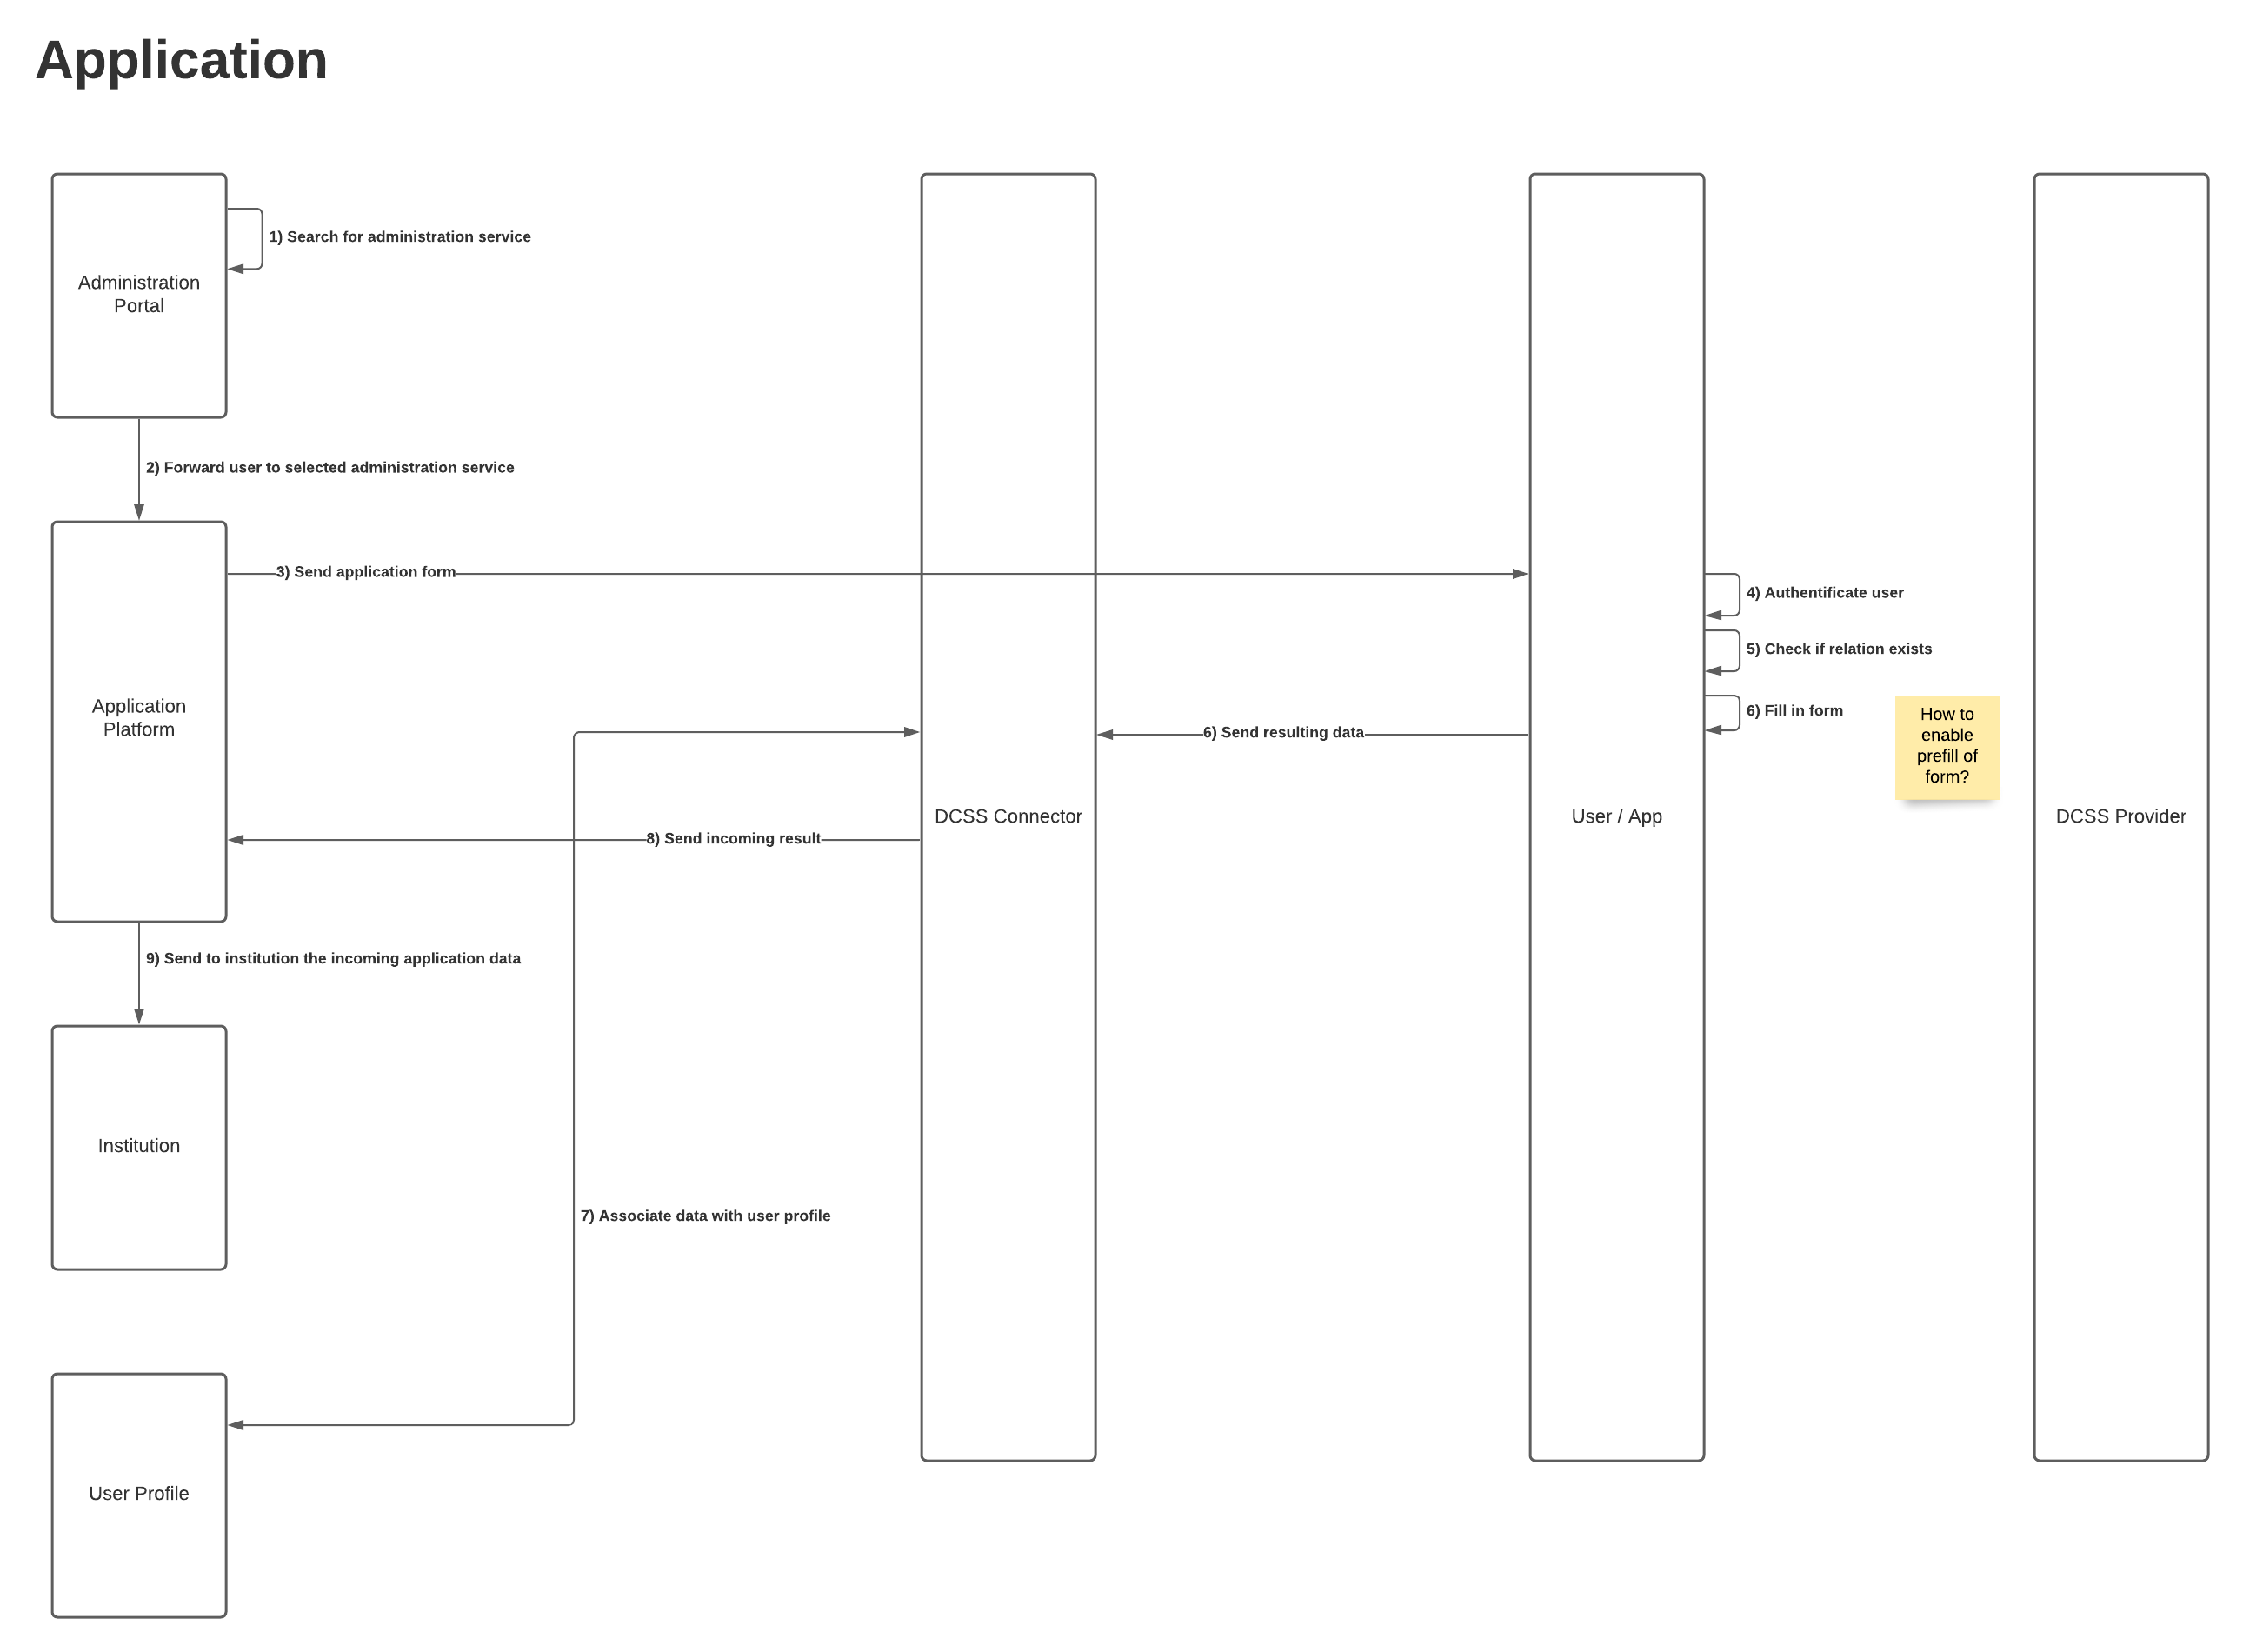
\includegraphics[width=\textwidth]{Basic Integration Application.png}

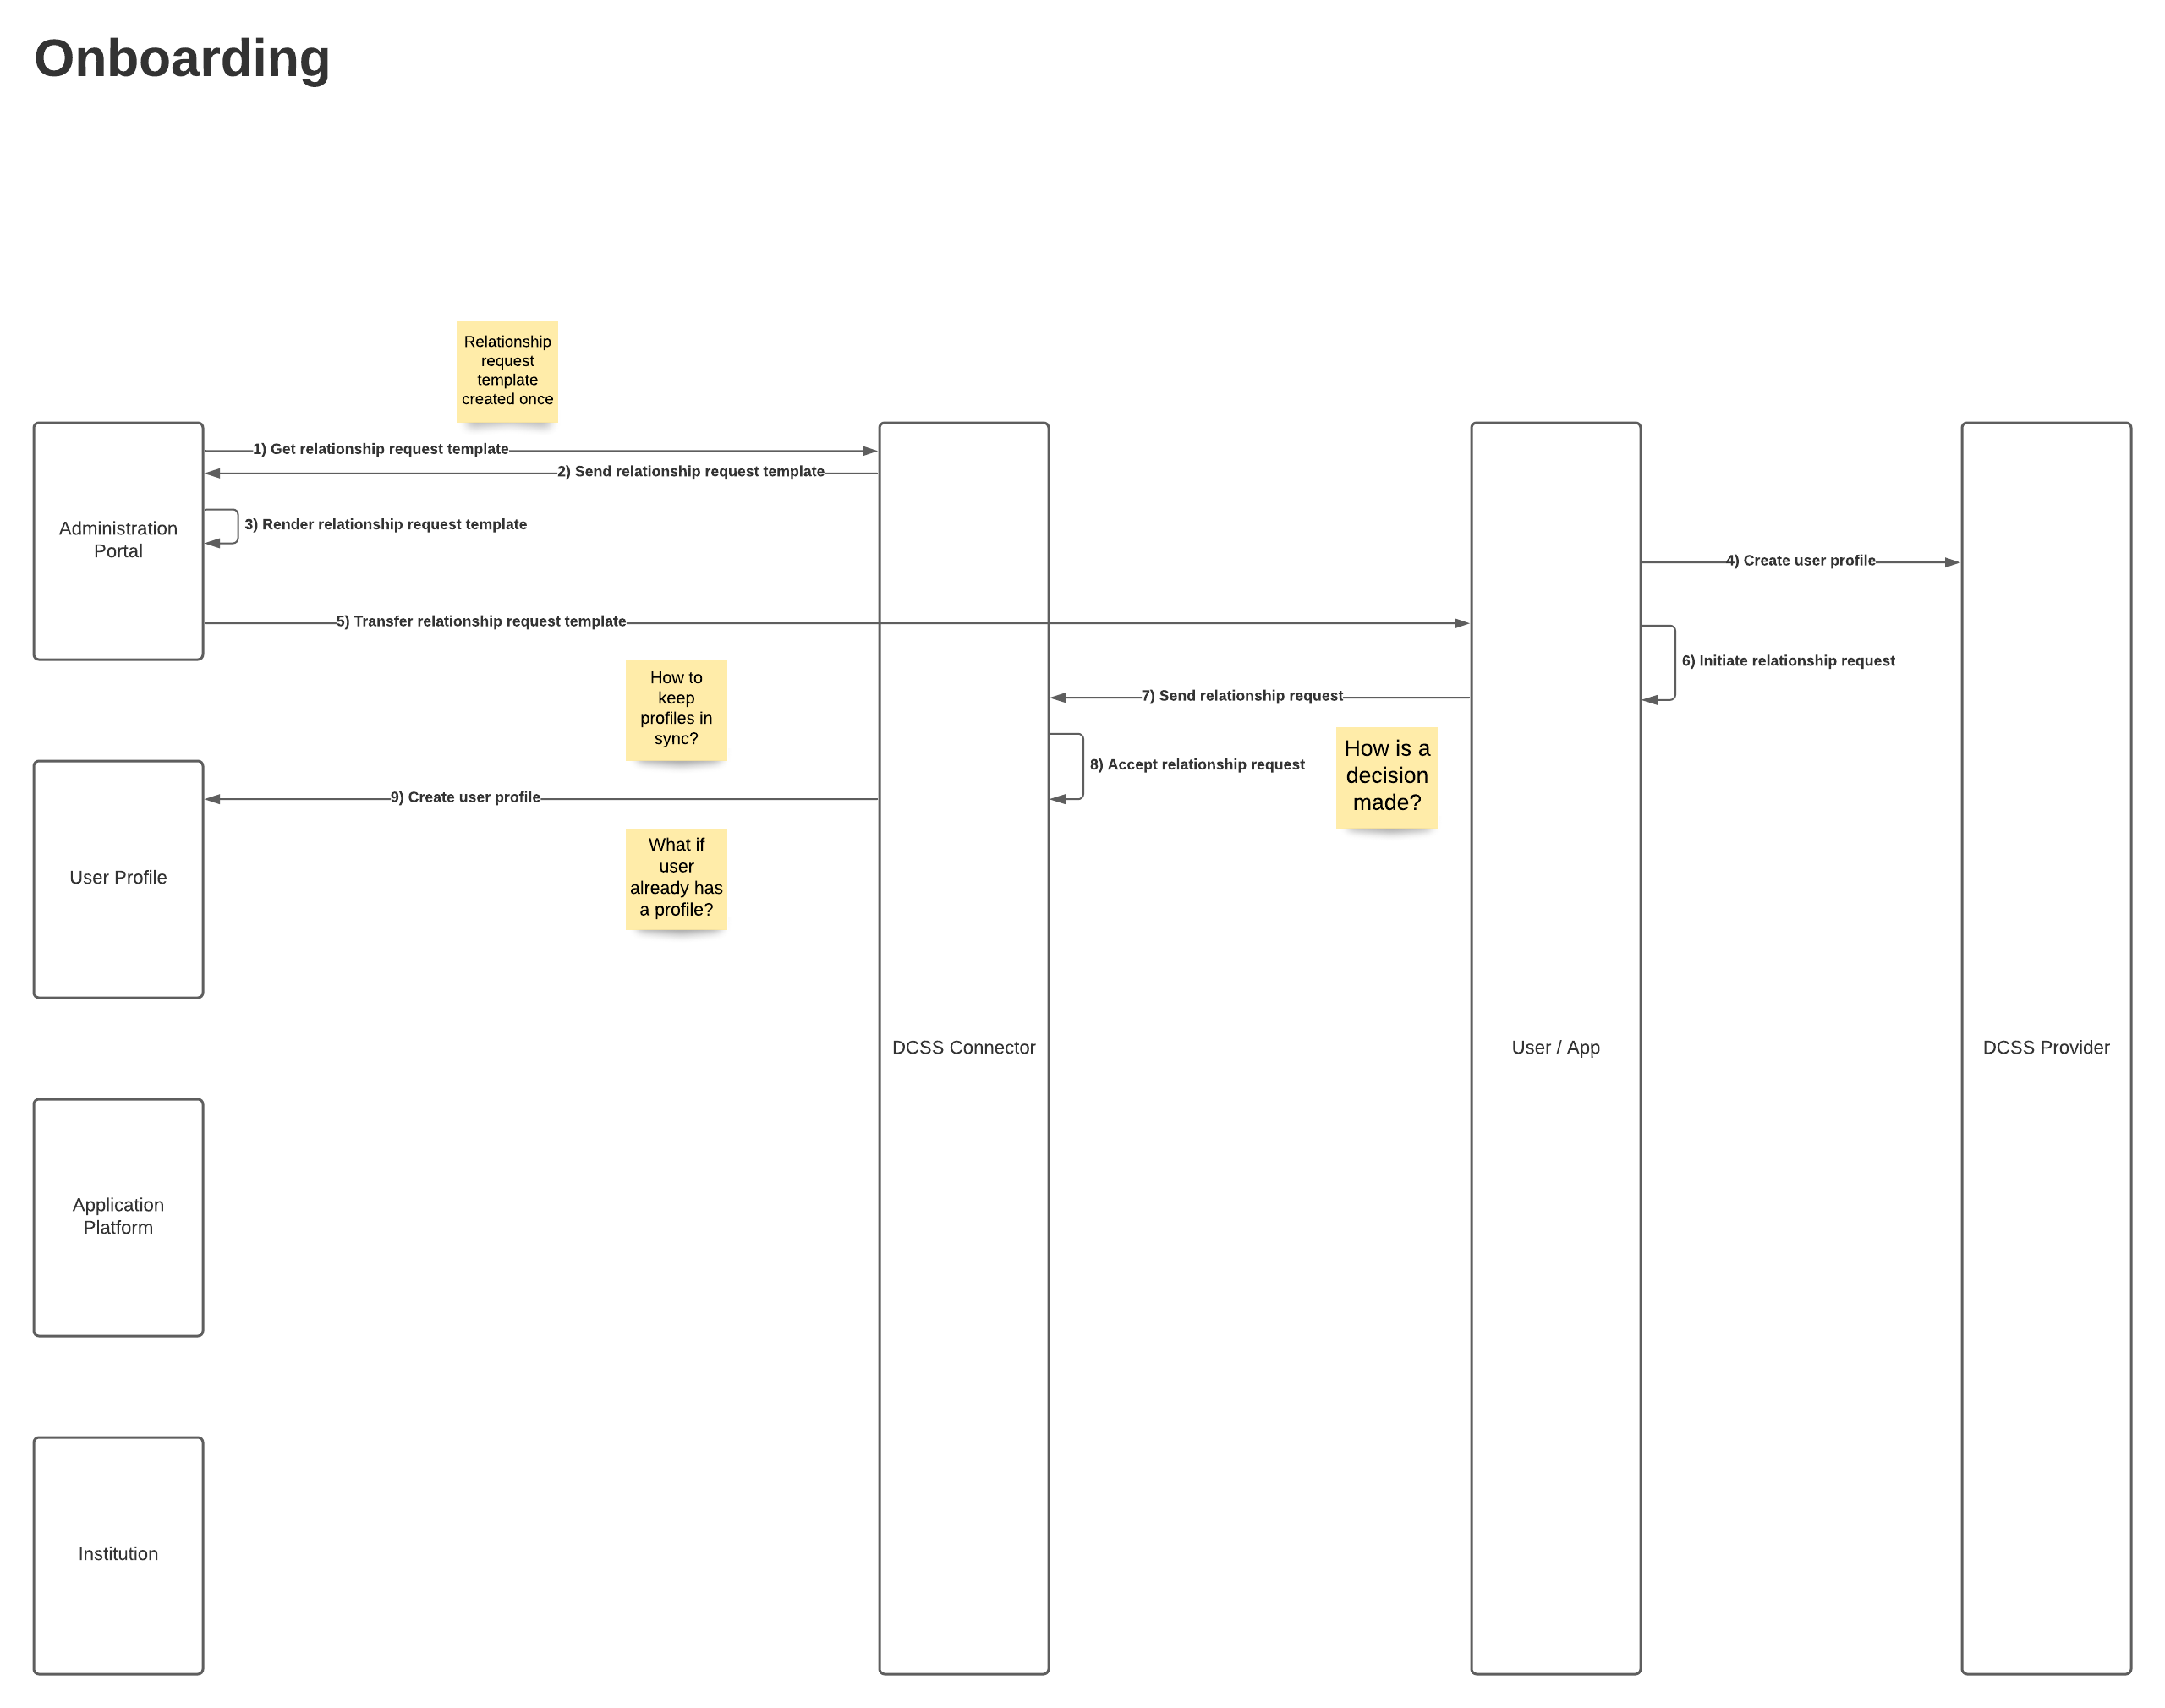
\includegraphics[width=\textwidth]{Basic Integration Onboarding.png}

\subsection{Messaging Integration}

\section{Advanced}

\subsection{Requirements}

\subsection{Flow Charts}

\subsection{Messaging Integration}


\chapter{Integration Architecture Evaluation}

\section{Technology}

\section{Customer Example}

\section{Operating Manual}

\chapter{Outlook}

\begin{itemize}
     \item Expanding integration architecture with capabilities for OSS scenarios of different areas than online administration self-service
     \begin{itemize}
          \item online payment self-service (PayPal, psd2)
          \item online shopping self-service (Amazon)
          \item online health care self-service (DVG)
          \item online entertainment self-service (Netflix, YouTube, Spotify)
          \item online information / support self-service (StackOverflow)
     \end{itemize}
\end{itemize}

\printbibliography


\end{document}
